\section{Clusteranalyse}

\subsection{Klassifizieren vs Clusteranalyse}

``Clusteranalyse'' und ``Klassifizierung'' m�gen auf den ersten Blick �hnlich erscheinen, aber es gibt einen wesentlichen Unterschied: Bei der Klassifizierung sind die Klassen vordefiniert und den Datens�tzen Klassen zugeordnet, w�hrend beim Clustering der Datensatz nach �hnlichen Merkmalen gruppiert wird, und es ist nicht erforderlich, dass Klassen vordefiniert wurden.

Um ein Clustering zu erreichen, werden �hnliche Objekte zusammen gruppiert, w�hrend un�hnliche Objekte voneinander getrennt werden. Gesucht sind also \(k\) Klassen \(K_1 \ldots K_k\), die alle Objekte richtig gruppieren.

\subsection{Zielsetzung beim Clustering}

\begin{itemize}
    \item In einem Datensatz wird nach der Mindestanzahl von Clustern gesucht.
    \item Objekte im selben Cluster m�ssen so �hnlich wie m�glich sein.
    \item Objekte im selben Cluster m�ssen so �hnlich wie m�glich sein.
    \item Eventuell sollten die Cluster auch hierarchisch geordnet werden k�nnen.
\end{itemize}

\subsection{Clusterbildungverfahren}

Bei der Auswahl von Merkmalen sollen die Merkmalen, die f�r alle Objekte auch Merkmalsauspr�gungen aufweisen werden, die mit vertretbarem Aufwand ermittelt werden k�nnen.

\paragraph{Typen von Merkmalen:}
\begin{itemize}
    \item Nominale Merkmale: z.B Namen, Farbe, \ldots
    \item Ordinale (geordnete) Merkmale: z.B Wochentage, Schulnoten, \ldots
    \item Metrische Merkmale: z.B Gr��e, Gewicht, Preis, \ldots
\end{itemize}

Die Clusteranalyse kann entweder hierarchisch oder durch Partitionierung angegangen werden. Beim hierarchischen Ansatz gibt es zwei M�glichkeiten: Top-Down, das mit einer Klasse beginnt, die sp�ter in mehrere Klassen aufgeteilt wird, oder Bottom-Up, das darin besteht, Klassen zusammenzufassen. Der Partitionierungsansatz gruppiert Objekte durch Umgruppierung. Jede Klasse hat einen vordefinierten "Kristallisationskern". Jedes neue Objekt wird anhand seiner Entfernung zum n�chsten Kristallisationskern eingeordnet.

\paragraph{Hierarchisches Clustering}

Beim hierarchischen Clustering geht es einfach darum, den Abstand zwischen Datenpunkten zu bestimmen und Objektpaare mit minimalen Abst�nden zwischen ihnen zu finden. Dies wird kontinuierlich durchgef�hrt, bis eine Hierarchie aufgebaut ist.

\begin{figure}[H]
    \centering
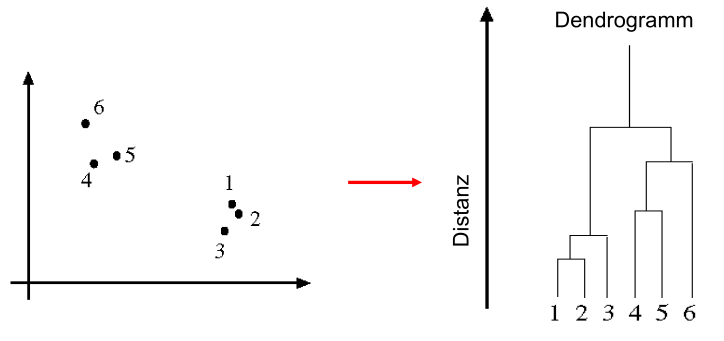
\includegraphics[width=0.9\textwidth]{figures/kap13/hierarchy-clustering.png}
    \caption{Hierarchisches Clustering}
    \label{fig:heirarchical-clustering}
\end{figure}

Beim hierarchischen Ansatz stellt sich die Frage, wie Klassen gruppiert werden k�nnen. Grundlage f�r dieses Verfahren ist die Bestimmung eines ``Klassenabstands''. Dies kann mit einigen Methoden erfolgen, z. B. mit der Next-Neighbour-Methode, mit der durchschnittlichen Entfernung zwischen Instanzen einer Klasse oder mit der Berechnung der Entfernung zwischen dem Mittelpunkt zweier Klassen.

\paragraph{K-Means clustering}

F�r den Partitionierungsansatz gibt es ein Verfahren, der als ``K-Means-Clustering'' bekannt ist. F�r diesen Ansatz wird die gew�nschte Anzahl von Klassen, \(k\), angegeben, in die der Datensatz gruppiert werden soll. Gehe dann wie folgt vor:

\begin{enumerate}
    \item F�r jeden Cluster wird ein Clusterschwerpunkt gew�hlt, der ein beliebiges Objekt oder keines der Objekte sein kann.
    \item Dann wird f�r alle Objekte der Abstand zwischen dem Objekt und dem n�chsten Cluster-Schwerpunkt berechnet. Jedes Objekt wird in dem Cluster eingeordnet, das den geringesten Abstand aufweist.
    \item Die Clusterzentrierung f�r alle Cluster wird dann neu berechnet.
    \item Die Schritte 2 und 3 werden wiederholt, bis die Clusterschwerpunkte stabil sind.
\end{enumerate}

